\subsection{Complejidad}
Para determinar la complejidad del algoritmo es necesario evaluar en primera instancia cuáles son las familias de casos en los cuales el algoritmo funciona peor en términos de eficiencia. Al ser una algoritmo de backtracking podado, concluimos que hallar una familia que cumpla con estas características es encontrar casos en donde las podas no tengan efecto, es decir, que no corten con las ramas de decisión tomadas. Analizándolo, determinamos que estos casos son aquellos en los cuales el algoritmo debe probar todas las combinaciones posibles y esto sucede en ejemplos como el siguiente:

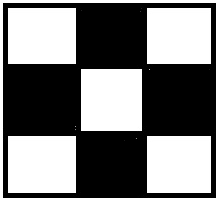
\includegraphics[scale=0.5]{ej3/imgs/ajedrezDibujo.png}

Como podemos observar, el hecho de que las paredes se encuentren ubicadas de esta forma me fuerzan a que las combinaciones que tenga que probar sean 4 por casillero porque colocar sensores en cualquier casillero libre no afecta a otros casilleros por el simple hecho de que los lasers emitidos no van a impactar en ninguno de ellos como consecuencia de las paredes. Es por esta razón que tendremos que probar $4^C$ combinaciones en donde C es la cantidad de casilleros libres.\footnote{notar que en caso de no tener podas el peor caso sería la matriz con todos casilleros libres y la complejidad se elevaría a $4^{n*m}$, donde (n*m)=tamaño de la matriz} Observando el gráfico se deduce que la cantidad de casilleros libres es la mitad de la cantidad de casilleros presentes, es decir, $(n*m)/2$.

Resumiendo, el algoritmo tendrá que realizar probar $4^{(n*m)/2}$ combinaciones en total en donde cada combinacion tiene un costo que esta determinado por complejidad de las operaciones que realizamos en cada llamada a la función Backtrack. Veamos cuál es el coste analizando el pseudocódigo:

\begin{algorithm}[H]
\caption{Backtrack}\label{Backtrack}
\begin{algorithmic}[1]
\Procedure{Backtrack}{$vector<int> casillerosUsados, int costo$}%\Comment{casillerosUsados: casilleros que fueron cubiertos hasta el momento, costo: dinero acumulado hasta el momento.}
	\State $vector<bool>\ casillerosUsadosViejo$ %\Comment{vector auxiliar para que sea posible volver a una rama anterior dentro de nuestro arbol de decisiones}
	\State $int\ aux$
	\If{$\neg hayMas(casillerosUsados)$}
		\If{$esSolucion() \wedge costo < \_costo$}
			\State $\_matrizRes=\_matriz$ % \Comment{guardo el resultado}
			\State $\_costo=costo $ %\Comment{actualizo el costo óptimo hasta el momento}
		\EndIf
	\Else
		\If{$costo<\_costo \wedge cumpleHastaElMomento(casillerosUsados)$}
			\State $casillerosUsadosViejo = casillerosUsados$ %\Comment{Guardo una copia antes de que sea modificado.}
			\ForAll{$c \in \_casilleros$}
				\If{$\neg usado(c,casillerosUsados)$}
					\ForAll{$s \in Sensores$}
						\If{$puedoColocarSensor(c,s,\_matriz)$}
							\State $InsertarSensor(c,s,\_matriz)$ 
							\State $marcarCasilleros(c,s,casillerosUsados)$
							\If{$esSensorBidireccional(s)$} 
								\State $backtrack(casillerosUsados,costo+4000)$
							\Else
								\State $backtrack(casillerosUsados,costo+6000)$
							\EndIf
							\State $sacarSensor(c,s,\_matriz)$ 
							\State $casillerosUsados=casillerosUsadosViejo$
						\EndIf
					\EndFor
					%\Comment{Caso en el que no se inserta ningún sensor.}
					\State $marcarCasillero(c,casillerosUsados)$
					\State $backtrack(casillerosUsados,costo)$
					\State $casillerosUsados=casillerosUsadosViejo$
				\EndIf
			\EndFor
		\EndIf
	\EndIf	
\EndProcedure
\end{algorithmic}
\end{algorithm}

Podemos decir que:

\begin{itemize}
	\item[1] hayMas(casillerosUsados) recorre el vector de casilleros Usados cuyo tamaño es la cantidad de casilleros simples de la grilla. Complejidad: $\mathcal{O}.((m*n)/2)$ (cantidad de casilleros de esta familia de casos)
	\item[2] esSolucion() verifica para cada uno de los casilleros simples si es apuntado por algun sensor. Verificar si es apuntado por un sensor cuesta $\mathcal{O}(1)$ ya que la función que se encarga de eso solo se mueve por la fila o columna de la matriz del casillero hasta encontrar una pared o el límite de la matriz y como mucho solo se va a mover un solo casillero. Complejidad: $\mathcal{O}((m*n)/2)$.
	\item[3] usado(c,CasillerosUsados) recorre el vector de casilleros usados. Complejidad: $\mathcal{O}((m*n)/2)$.
	\item[4] puedoColocarSensor(c,s,$\_$matriz) verifica si hay algun sensor en la columna o fila donde se va a colocar el sensor lo cual es $\mathcal{O}(1)$ ya que al igual que en el caso de esSolucion() va a moverse solo un casillero por la presencia de una pared o límite de la matriz. Complejidad: $\mathcal{O}(1)$.
	\item[5] InsertarSensor(c,s,$\_$matriz) es $\mathcal{O}(1)$ ya que simplemente se inserta en la coordenada c de la matriz un valor númerico que identifica a un laser.
	\item[6] marcarCasilleros(c,s,casillerosUsados) recorre el vector de casilleros usados. Complejidad: $\mathcal{O}((m*n)/2)$.
	\item[7] sacarSensor(c,s,$\_$matriz) es $\mathcal{O}(1)$ ya que simplemente se inserta en las coordenada c de la matriz un valor númerico.
\end{itemize}

Los items 4,5,6 y 7 se encuentran dentro de un for que recorre todos los casilleros simples por lo cual la complejidad de ese pedazo será: $\mathcal{O}((m*n)/2)$ * ($\mathcal{O}(1)$ $+$ $\mathcal{O}(1)$ $+$ $\mathcal{O}((m*n)/2)$ $+$ $\mathcal{O}(1)$ ).

Por lo tanto la complejidad de cada pasada del Backtrack es:
$\mathcal{O}((m*n)/2)$ $+$ $\mathcal{O}((m*n)/2)$ + $\mathcal{O}((m*n)/2)$ $+$ $\mathcal{O}((m*n)/2)$ * ($\mathcal{O}(1)$ $+$ $\mathcal{O}(1)$ $+$ $\mathcal{O}((m*n)/2)$ $+$ $\mathcal{O}(1)$ ) = $\mathcal{O}((m*n)/2)$ $*$ $\mathcal{O}((m*n)/2)$

En conclusión, la complejidad total del algoritmo es:

$\mathcal{O}(4^{((m*n)/2)}*((m*n)/2))^2$
